\documentclass{article}

% Packages
\usepackage{amsmath} % For math equations
\usepackage{amssymb} % For math symbols
\usepackage{geometry} % For page layout
\usepackage{fancyhdr} % For headers and footers
\usepackage{lipsum} % For dummy text (remove this line)
\usepackage{float}
\usepackage{listings}
\usepackage{xcolor}
\usepackage{graphicx}
\usepackage{array} % 导入 array 宏包
\usepackage{verbatim} % 导入 verbatim 宏包
\usepackage{calc}
\usepackage{slashbox}
\usepackage{pict2e}
\usepackage[utf8]{inputenc}
\usepackage{circuitikz}

% Set the page margins
\geometry{margin=1in}
% Set the top margins
\addtolength{\topmargin}{-.5in}
\title{Digital System Assignment 4}
\author{He Tianyang}
\date{\today}

\begin{document}
\maketitle

\section{Problem 1}
\textbf{Solve:}

The circuit diagram can be described as follow logic expression:
\begin{equation}
    \begin{aligned}
        Y & =  \overline{\left(\overline{A\overline{B}}\cdot \overline{BC} \cdot\overline{\overline{A}C}\right)} \\
          & =A\overline{B}+BC+A\overline{C}                                                                      \\
          & = A+BC
    \end{aligned}
\end{equation}

Therefore, we can draw the K-map for the logic expression:
\begin{table}[H]
    \centering
    \begin{tabular}{|c|c|c|c|c|}
        \hline
        \backslashbox{A}{BC} & 00 & 01 & 11 & 10 \\
        \hline
        0                    & 0  & 0  & 1  & 0  \\
        \hline
        1                    & 1  & 1  & 1  & 1  \\
        \hline
    \end{tabular}
\end{table}

From the K-map, we can see that when the input changes from 011 to 110 or 101, if all the ABC change at the same time, there is no any race condition.

if changes like:
\begin{equation*}
    011\rightarrow 010\rightarrow 110
\end{equation*}

or

\begin{equation*}
    011\rightarrow 001\rightarrow 101
\end{equation*}

there will be a 0 output in this process, and \textbf{functional hazard will occur}.\\

To avoid the functional hazard, we can add a optional gate to the output of the circuit, which closed when the input signal changes and opened when the inputs are stable. or add a filter capacitor to the output of the circuit.


\section{Problem 2}

The waveform of the circuit is shown in the Figure.\ref{fig:waveform} below
\begin{figure}
    \centering
    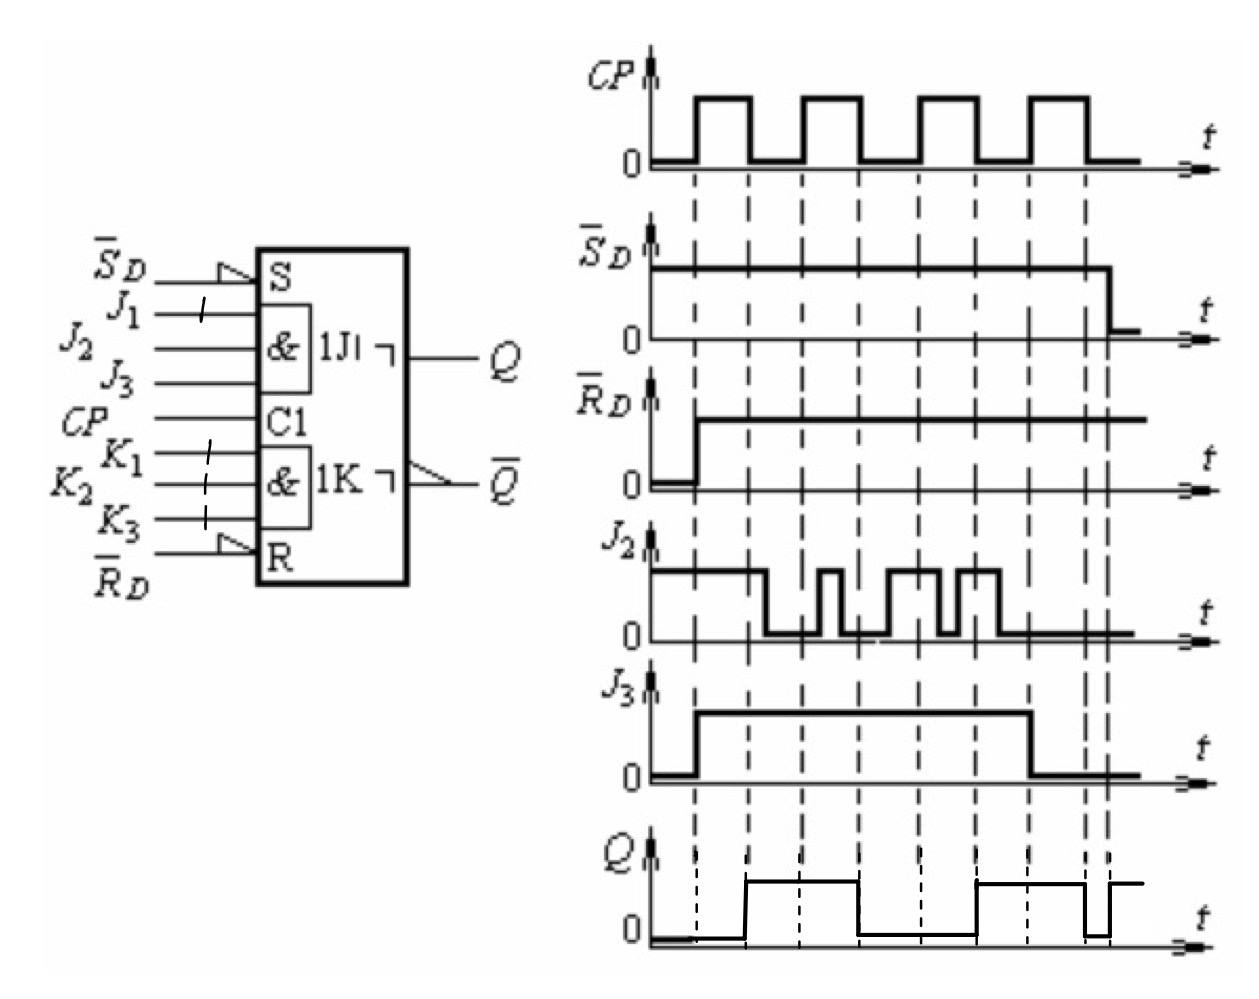
\includegraphics[width=0.8\textwidth]{./image/waveform.jpg}
    \caption{Waveform of the circuit}
    \label{fig:waveform}
\end{figure}

\end{document}